\section{Electric charge neutrality}
\label{section: charge neturality}


A pion condensate will have an electric charge.
In the grand canonical ensemble, the QCD Lagrangian will have the term  $\mu_Q e\bar q \gamma^0 Q q$, where $e \bar q \gamma^\mu Q q$ is the electric current density, $Q$ the quark charge matrix \autoref{three-flavor charge matrix}, and $e \mu_Q = \mu_I + 2 \mu_S$ is the electric charge chemical potential.
In the case of $\mu_S = 0$, the charge density is
%
\begin{equation}
    n_Q = - \pdv{\Eff}{\mu_Q} = e n_I.
\end{equation}
%
A realistic astrophysical object will not have a macroscopic electric charge.
Therefore, we will model pion stars with the additional constraint of charge neutrality by including charged leptons in the form of muons or electrons.
These leptons are free fermions, with an electric charge of $- e$.
We may therefore use the results from \autoref{section: cold fermi star} and \autoref{section: fermions}.
The electric charge density of the leptons is given $- e n_\ell$, where $n_\ell$ is the particle number and, in this case, the lepton number.
In \autoref{Fermi gas particle density}, we found the expression
%
\begin{equation}
    \label{lepton density}
    n_{\ell} = \frac{8}{3} 
    \frac{u_{\ell, 0}}{m_\ell} x_f^3,
\end{equation}
%
where $x_f = \sqrt{ {\mu_\ell^2}/{m_\ell^2} - 1}$ is the dimensionless Fermi momentum, $m_\ell$ the lepton mass, and $\mu_\ell$ the lepton chemical potential.
This formula is valid for $\mu_\ell \geq m_\ell$.
We have introduced the characteristic energy density of leptons,
%
\begin{equation}
    u_{\ell, 0} = \frac{m^4_\ell}{8 \pi^2}.
\end{equation}
%
The criterion for charge neutrality is then
%
\begin{equation}
    \label{criterion charge neutrality}
    n_I = n_\ell.
\end{equation}
%
With this, we can determine the lepton chemical potential as a function of the isospin chemical potential, $\mu_\ell = \mu_\ell(\mu_I)$.
The leading order result for the isospin density of the pion condensate is given in \autoref{isospin density}.
Inserting the expressions for these densities into \autoref{criterion charge neutrality}, we get
%
\begin{equation}
    \label{equation mu ell mu I}
    A \left(\frac{\mu_\ell^2 }{m_\ell^2} - 1 \right)^{3/2}
    = \frac{\mu_I}{m_\pi}\left( 1 - \frac{m_\pi^4}{\mu_I^4}  \right).
\end{equation}
%
Both densities vanish at the point $(\mu_I, \mu_\ell) = (m_\pi, m_\ell)$, which we have seen earlier is the point where the pressure and energy density of both the Fermi gas and the pion condensate vanish.
We have introduced the dimensionless constant
%
\begin{equation}
    A = \frac{8}{3} \frac{m_\pi} {m_\ell} \frac{u_{0, \ell}}{u_0}
    = \frac{1}{3 \pi^2} \frac{m_\ell^3}{m_\pi f_\pi^2}.
\end{equation}
%
Setting the lepton mass equal the electron mass or muon mass gives, respectively, $A = 3.9 \times10^{- 9}$ and $A = 3.5 \times 10^{-2}$.
In this case, we can write the expression for $\mu_\ell(\mu_I)$ as an explicit function,
%
\begin{equation}
    \label{mu ell from mu I}
    \frac{\mu_\ell}{m_\ell}
    =
    \sqrt{
        1 + A^{-2/3}
        \left[
            \frac{\mu_I}{m_\pi}\left( 1 - \frac{m_\pi^4}{\mu_I^4}  \right)
        \right]^{2/3}
    }.
\end{equation}
%
These relationships are illustrated in \autoref{fig: chemical potentials}.
The plot on the left is the electron chemical potential as a function of isospin chemical potential, both normalized to the masses of their corresponding particles, while the muon chemical potential is on the right.
We see that both lepton potentials are suppressed, relative to the isospin chemical potential, by the $A$ constant in \autoref{equation mu ell mu I}.
The electron is much lighter than the pion, and therefore grows much faster than the muon chemical potential.

\begin{figure}[!htb]
    \centering
    \begin{subfigure}{0.49 \textwidth}
        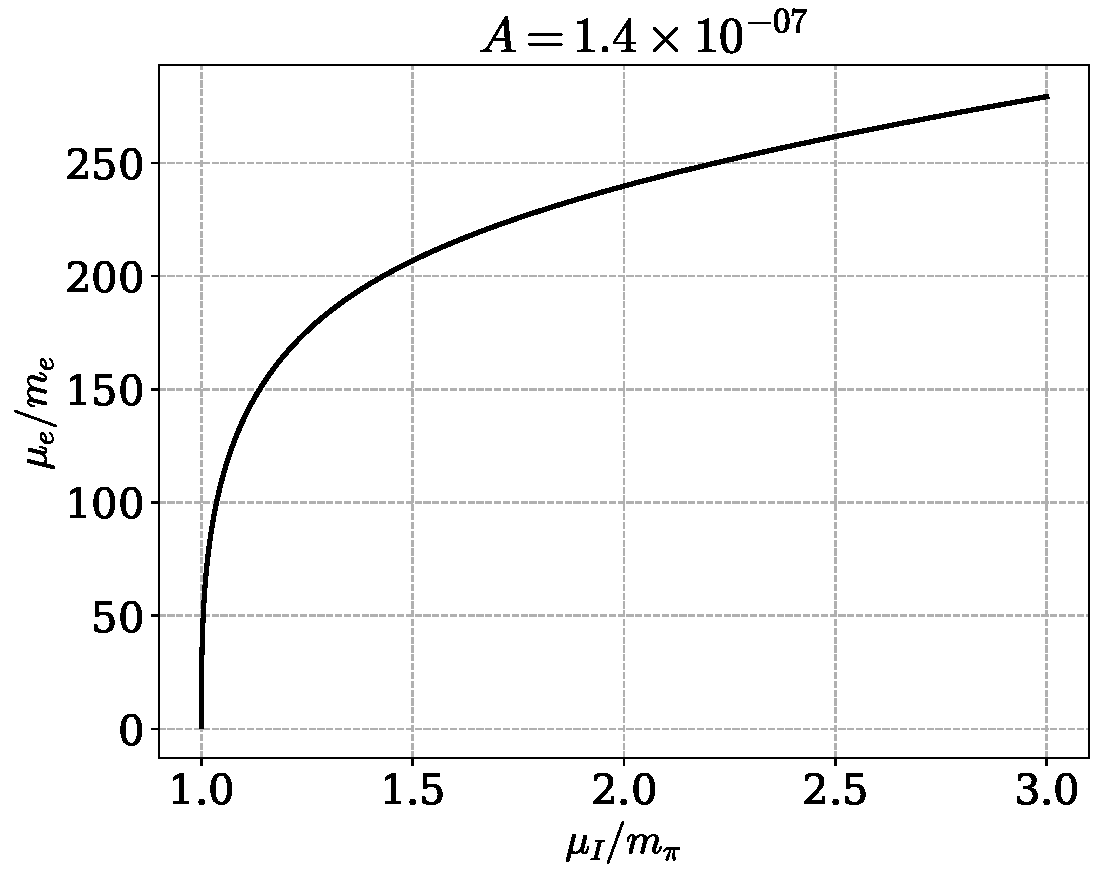
\includegraphics[width=\textwidth]{../scripts/figurer/charge_neutrality/chemical_potential_e.pdf}
    \end{subfigure}
    \begin{subfigure}{0.49\textwidth}
        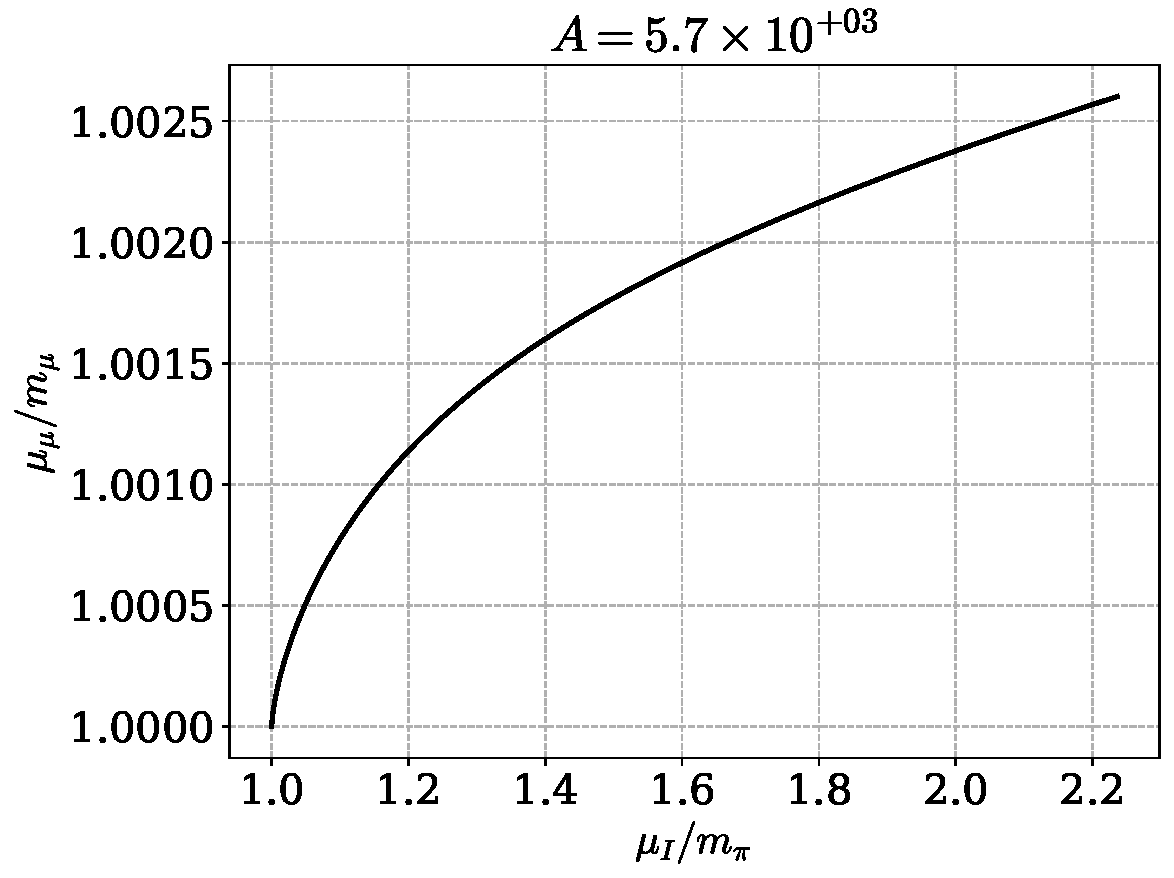
\includegraphics[width=\textwidth]{../scripts/figurer/charge_neutrality/chemical_potential_mu.pdf}
    \end{subfigure} 
    \caption{
        The lepton chemical potentials as functions of the isospin chemical potential normalized to their respective particles masses.
        The electron chemical potential is shown to the left, the muon to the right.
    } 
    \label{fig: chemical potentials}
\end{figure}


The total pressure and energy density will now be the sum of the contributions from the pion condensate and the leptons.
The lepton contribution to these, which we found in \autoref{Fermi gas energy density} and \autoref{Fermi gas pressure}, is
%
\begin{align}
    u_\ell 
    &= u_{\ell,0} 
    \left[(2x_f^3 + x_f) \sqrt{1 + x_f^2} - \arcsinh\left(x_f\right)\right], \\
    p_\ell
    &=\frac{1}{3} u_{\ell,0}
    \left[(2x_f^3 - 3x_f) \sqrt{1 + x_f^2} + 3\arcsinh\left(x_f\right)\right].
\end{align}
%
The contribution from the pion condensate is, as we found in \autoref{pressure leading order chpt} and \autoref{energy density leading order chpt},
%
\begin{align}
    u_\pi &= \frac{1}{2} u_0 \left( \frac{\mu_I}{m_\pi} - \frac{m_\pi}{\mu_I}\right)^2 \\
    p_\pi &= \frac{1}{2} u_0 \left( 2 + \frac{\mu_I^2}{m_\pi^2} - 3 \frac{m_\pi^2}{\mu_I^2}  \right)
\end{align}
%
This leads to a total pressure and energy
%
\begin{equation}
    p = p_\pi + p_\ell, \quad u = u_\pi + u_\ell.
\end{equation}
%
As \autoref{criterion charge neutrality} gives $\mu_\ell$ as a function of $\mu_I$, these are both parametrized by the isospin chemical potential, and we can extract the equation of state $u = u(p)$.
The full equation of state in different regimes is shown in \autoref{fig: eos with leptons}.
On the top left, the addition of the electron results in a much stiffer equation of state than the addition of the muon.
We have seen that the low-pressure energy density of the pion is $m_\pi n_I $, while for the lepton it is $m_\ell n_\ell$.
As $n_I = n_\ell$, the low pressure limit of the energy of the energy density is $(m_\pi + m_\ell)n_ I$, which explains why the muon, where $m_\mu \approx m_\pi$, contributes a lot more to the energy density than the electron, for which $m_e \ll m_\pi$.
On the top right, we see that the pressure regime is dominated by the pion contribution.
However, as chiral perturbation assumes small pion energies and small external currents, this result must be used carefully.
On the bottom, the equation of state in an intermediate range is shown.
It is not very sensitive to the mass of the lepton, at least as long as it is less than the pion mass.

\begin{figure}
    \centering
    \begin{subfigure}{0.49\textwidth}
        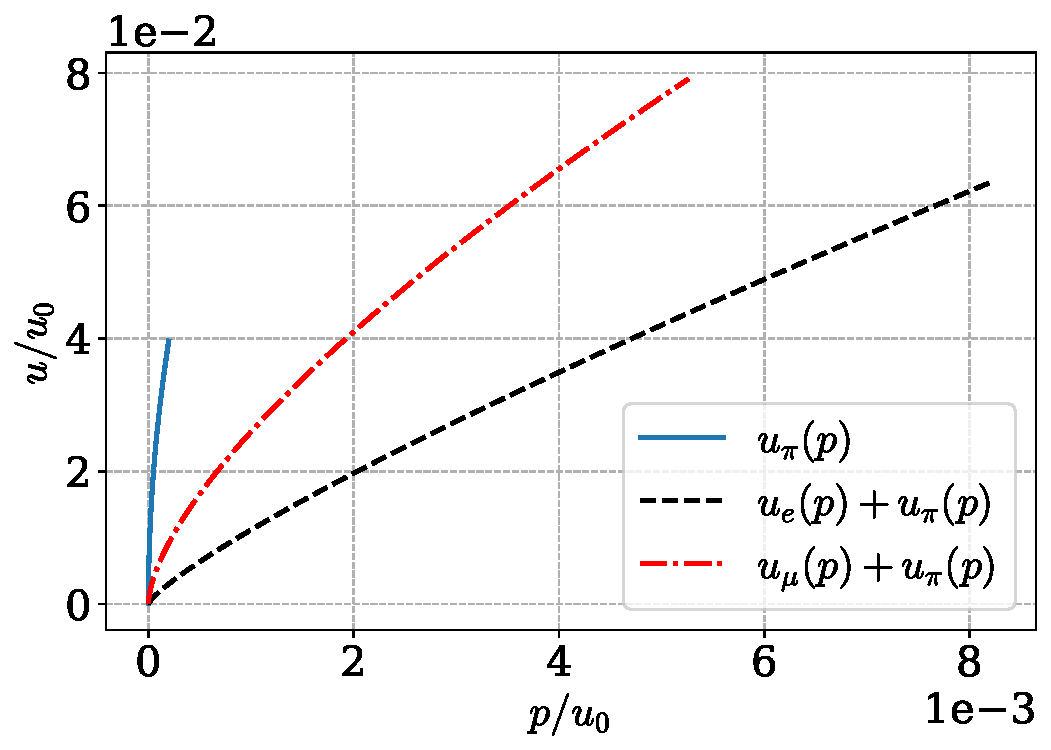
\includegraphics[width=\textwidth]{../scripts/figurer/charge_neutrality/eos_nr.pdf}
    \end{subfigure}
    \begin{subfigure}{0.49\textwidth}
        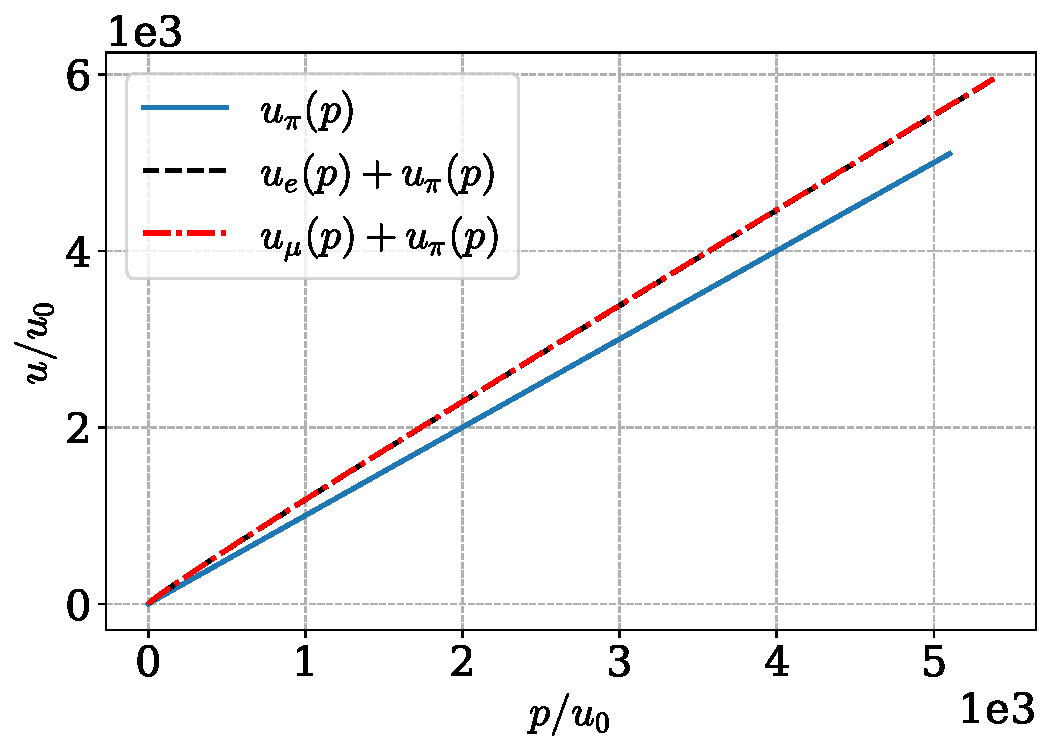
\includegraphics[width=\textwidth]{../scripts/figurer/charge_neutrality/eos_ur.pdf}
    \end{subfigure}
    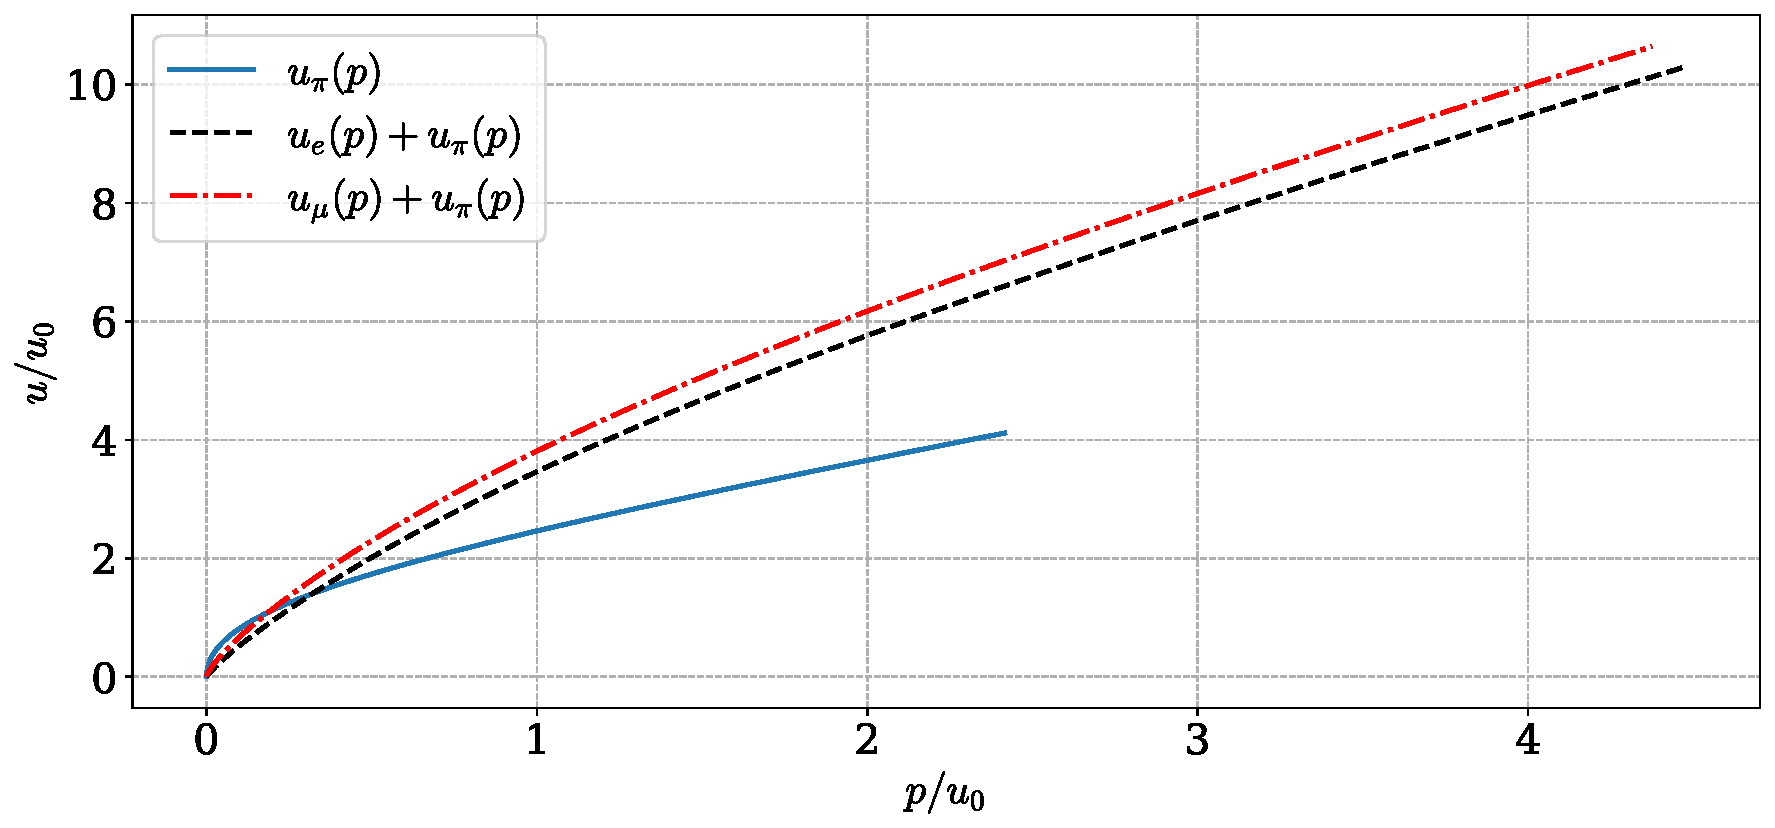
\includegraphics[width=\textwidth]{../scripts/figurer/charge_neutrality/eos_I.pdf}
    \caption{
        The equation of state including a lepton is compared with the equation of state of only the pion condensate in two different regimes.
        The pressure and energy density is normalized to $u_0 = f_\pi^2 m_\pi^2$.
    }
    \label{fig: eos with leptons}
\end{figure}

We can find the ultrarelativistic limit by letting $\mu_I^2/m_\pi^2 = y$, $y \gg 1$.
From \autoref{mu ell from mu I}, we find that the lepton chemical potential to leading order in $y$ is $\mu_\ell^2 \propto y^{1/3}$.
In \autoref{section: cold fermi star}, we found that in the ultrarelativistic limit of non-interacting fermions, both the pressure and energy is proportional to $x_f^4 \propto y^{2/3}$.
In the case of the pion, however, both are proportional to $\mu_I^2 \propto y$.
Therefore, the ultrarelativistic limit of the combined system is, to leading order, given by the ultrarelativistic limit of the pion condensate alone.

As before, we can find the non-relativisitic limit by letting $\mu_I^2/m_\pi^2 = 1 + \epsilon$.
Inserting this into \autoref{mu ell from mu I} and expanding to first order in $\epsilon$, we get $\mu_\ell = 1 + (2 A^{-1} \epsilon)^{2/3} $.
This is equivalent to $x_f = (2 A^{-1} \epsilon)^{1/3} $.
In \autoref{section: cold fermi star}, we found the non-relativistic limit of the pressure and energy of the Fermi gas, i.e., the lowest order contribution in $x_f$, as $x_f \rightarrow 0$.
Inserting this new result into these limits, we get the leading low energy limits of the pressure and energy, 
%
\begin{equation}
    u_{\ell, \text{nr}} = \frac{8}{3} \frac{2}{A} u_{\ell,0} \epsilon, \quad
    p_{\ell, \text{nr}} = \frac{8}{15} \left(\frac{2}{A} \right)^{5/3}  u_{\ell,0}  \epsilon^{5/3}.
\end{equation}
%
From \autoref{section: thermodynamics leading order}, we have the equivalent expressions for the pion condensate,
%
\begin{equation}
    u_{\pi, \text{nr}} = 2 u_0 \epsilon, \quad p_{\pi, \text{nr}} = \frac{1}{2} u_0 \epsilon^2.
\end{equation}
%
As we see, the energy density of the pion condensate and the leptons are of the same order, and both will therefore contribute to the leading order energy density.
However, the lepton pressure is of a lower order, and \emph{only} this will contribute to the leading order pressure.
At low enough isospin chemical potential, then, the leading order behavior of the combined system is
%
\begin{equation}
    u_{\text{nr}} 
    = 2 u_0 \left(1 + \frac{1}{2}\frac{m_\ell}{m_\pi} \right)  \epsilon, \quad
    p_{\text{nr}} = \frac{8}{15} u_{\ell,0} \left(\frac{2}{A} \right)^{5/3} \epsilon^{5/3}.
\end{equation}
%
The equation of state is now a polytrope with $\gamma = \frac{5}{3}$, different from the $\gamma = 2$ polytrope of only the pion condensate.
For a heavy lepton, $m_\ell \gg m_\pi$, the factor $\smash{A^{-\frac{5}{3}}}$ would suppress leading order the lepton contribution to the pressure.
Thus, the equation of state would have an intermediate range in which it would be well approximated as a polytrope with $\gamma = 2$, and a modified poly tropic constant $K'^{-1} = 8 (1 + \frac{1}{2} m_\ell/m_\pi)^2$.
The full equation of state is compared to the non-relativisitic limit in \autoref{fig: lepton eos limit}.

\begin{figure}[!htb]
    \centering
    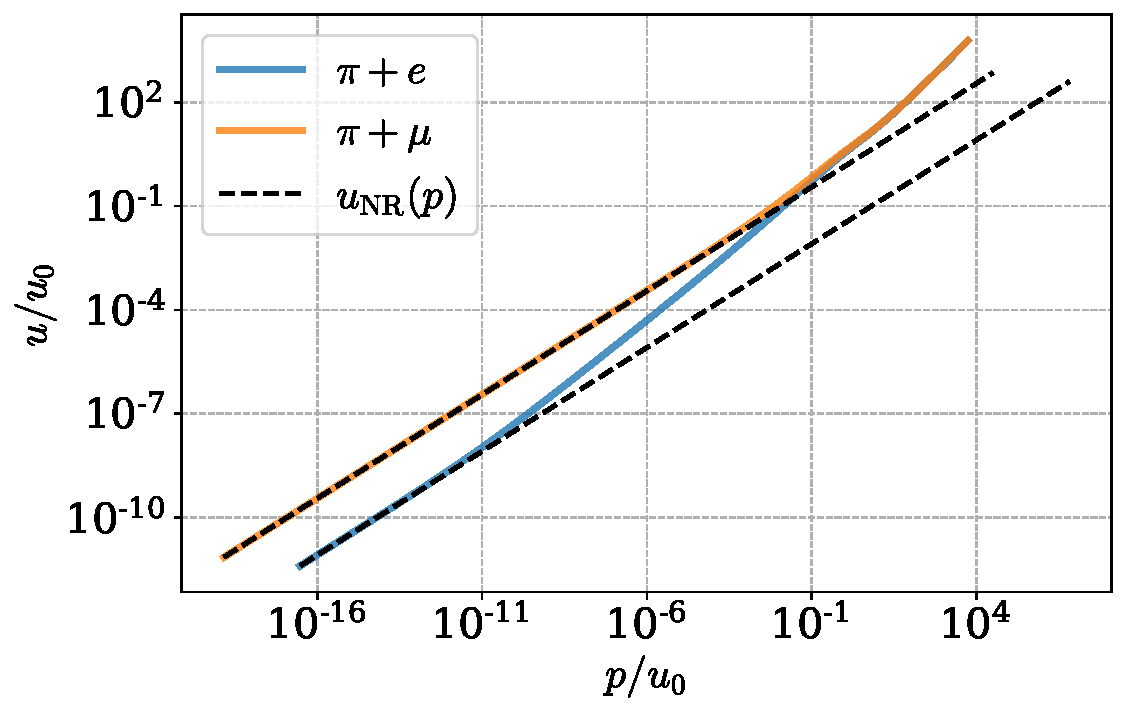
\includegraphics[width=\textwidth]{../scripts/figurer/charge_neutrality/eos_lim.pdf}
    \caption{
        The full equation of state of the pion + lepton systems, compared with the non-relativistic limit.
        Both the energy density and the pressure is given in units of $u_0 = m_\pi^2 f_\pi^2$.
    }
    \label{fig: lepton eos limit}
\end{figure}
